\documentclass[10pt,a4paper,hidelinks]{article}
\usepackage[utf8]{inputenc}
\usepackage[english]{babel}
\usepackage[T1]{fontenc}

\newcommand{\documentStatus}{DRAFT}


\usepackage{amsmath}
\usepackage{amsfonts}
\usepackage{amssymb}
\usepackage{graphicx}
\usepackage{lmodern}
\usepackage{tikz}
\usetikzlibrary{positioning}
\usepackage{epigraph} 
\usepackage[left=2.5cm,
            right=2.5cm,
            top=2cm,
            bottom=2cm]{geometry}
\usepackage{setspace}
\usepackage{caption}
\usepackage{subcaption}
\usepackage{epigraph}
\usepackage{pdflscape}

\usepackage{titlesec}
\usepackage{tcolorbox}
\usepackage{background}
\usepackage{url}
\usepackage[pdfauthor={Pierre Jézégou},
            pdftitle={ADS assignement},
            pdfsubject={Word games},
            pdfkeywords={}]{hyperref}
\usepackage{wrapfig}


\backgroundsetup{contents=\documentStatus, color=\watermarkColor}

\usepackage{fancyhdr}
\usepackage{textpos}
\usepackage{sectsty}
\usepackage{xcolor}

\setlength{\parindent}{0pt}

%%%%%%%%%%%%%%% Colors %%%%%%%%%%%%%%%
\subsectionfont{\color{fib_red}}
\subsubsectionfont{\color{fib_gray}}
\renewcommand\fbox{\fcolorbox{black}{fib_red!20}}

\definecolor{fib_red}{RGB}{191,21,64}
\definecolor{fib_gray}{RGB}{111,111,111}


\usepackage[Bjornstrup]{fncychap}
\newcommand{\watermarkColor}{red!10}


\onehalfspacing


\newcommand\VRule[1][\arrayrulewidth]{\vrule width #1}
\usepackage{xcolor,colortbl}

\newtcolorbox{mybox}[1]{
    arc=0pt,
    boxrule=0pt,
    colback=#1,
    width=\linewidth,
    halign=left,
}

\newenvironment{framed}[2]{
    \vspace*{0.5em}
    \begin{mybox}{orange!10}
        \textbf{#1} :\hfill \textit{#2}\\
        \hrule\vspace*{1em}
}
{\end{mybox}}

\newenvironment{exercise_description}[1]{
    \begin{framed}{Exercice description}{#1}
}
{\end{framed}}

\usepackage{lmodern}
\renewcommand*\familydefault{\sfdefault}


\fancyfoot[R]{\raisebox{-0.5\baselineskip}{\includegraphics[scale=0.25]{images/logos/upc_logo.jpeg}}}

\begin{document}
\pagestyle{plain}
\backgroundsetup{contents=,color=red!30}
\pagecolor{white}

\begin{center}
    \color{red!50!white}
    \textbf{\huge{STATUT - \documentStatus}}
\end{center}

\vfill

\color{black}
\begin{center}
    % \includegraphics[width=0.5\linewidth]{images/logos/fib.png} \\
    \includegraphics[height=2cm]{images/logos/upc_logo.jpeg} \\
    \vfill

    \rule{\linewidth}{0.5mm} \\[1cm]
    {\Huge \textsc{\textcolor{fib_red}{Word Games}}}\\[1cm]
    {\Large \textsc{Assignment}}\\[0.4cm]
    {\huge \textsc{\textbf{Advanced data structures}}}\\[1cm]
    {\Large \textsc{Master in Research and Innovation - UPC}}\\[0.4cm]
    \rule{\linewidth}{0.5mm} \\[1.5cm]
\end{center}

\vfill

\textbf{Authors :}
\begin{itemize}
\item Pierre \textsc{Jézégou}\newline
\textit{(Engineering student at École Centrale de Lille, Exchange student at UPC)}
\end{itemize}

\vfill

\newpage
\color{black}
\pagecolor{white}
\pagestyle{fancy}
\tableofcontents

\section{Introduction}
This program implements a trie data structure to store words.
A trie is a tree-like data structure that stores a dynamic set of strings, where each node represents a single character of the string.
The TrieNode class represents the structure of a trie node, which contains information such as its children, whether it marks the end of a word, its value (character), and its depth in the trie.\\

The Trie class implements the operations and building procedure for the trie. It has methods to insert words into the trie and to search for words in the trie.
The program also includes functions to generate TikZ code for visualizing the trie. The \verb|generate_tikz_trie| function generates TikZ code to visualize the trie structure, while the \verb|generate_search_path| function generates TikZ code to visualize the search path for a given word in the trie.
Finally, the program creates an instance of the Trie class, inserts words from a given dictionary into the trie, and generates TikZ code to visualize the trie with a specific search word highlighted.\\

L'ensemble du code source (programmes, documentation et générateurs d'image) est disponible dans le respository GitHub dédié au projet : \url{https://github.com/pierre-jezegou/word-game}\\

For performance testing of algorithms, we use a MacBook Air with the M2 processor. This hardware provides ample computing power to execute our algorithms efficiently, ensuring swift analysis of their performance.

Comme conseillé, ce rapport a été rédigé en \LaTeX

\section{Word Challenge}
\begin{exercise_description}{Word challenge}
    In Word Challenge the user gives a (multi)set of up to 17 letters, and the program produces all words which can be written using a subset of the given letters. For example, if the user gives the letters \verb|{E,T,F,H,R,R,E,O,E}| the program will write by increasing length and then in alphabetic order all the words that can be built using (some) of these letters, for example, \verb|FOR, HER, ORE, THE, .., HERE, ..., THEREFORE|. The dictionary does only contain words of $\text{length}\geqslant  3$, hence if given $\ell \geqslant 3$ the list of results starts with words of length 3 and ends with words of length $\ell$ (or smaller, if there were no words of length $\ell$ using all given letters). Besides being able to play interactively with the user, the program must give an "automatic mode" in which the program does the following repeatedly:
    \begin{enumerate}
    \item Picks a random word from the dictionary of given length $\ell$
    \item Rearranges its letters randomly
    \item Supplies these letters to the function that generates the list of words which can be built from the given letters
    \end{enumerate}
    In automatic mode the user gives the number of times that the game will be played, and the length $\ell$, and it outputs the average number of words found and the average CPU time that the program takes to "solve" a word of length $\ell$.
\end{exercise_description}


\subsection{Implement \type{trie} data structure}
Dans un premier temps, nous choisissons d'appuyer cet exercice sur une structure bien connue dans l'utilisation de chaînes de caractère : les tries. Cela nous permettra ainsi de stocker les mots de manière structurée et de les récupérer avec une complexité moindre (justifée plus tard).\\

Cette structure s'appuiera sur deux classes \textit{Python} pour modéliser le trie lui même (\type{Trie}) et les noeuds du \textit{trie} \type{TrieNode}. Chacune de ces deux structures de données seront dotées de paramètres et de méthodes permettant la résolution du travail de manière optimale.

\subsubsection{\type{TrieNode} data structure}
\begin{figure}[h]
    \centering
    \begin{tikzpicture}
        \node[draw, rounded corners=2mm, inner sep = 0.2cm, fill=orange!0] { 
        \begin{tikzpicture} 
            \node[inner sep = 1mm] (title) { \Large{\bfseries TrieNode }}; 
            % \draw (title.south west) -- (title.south east);
            \node[at=(title.south), anchor=north, inner sep=3mm, align=left, fill=green!30!black!10, yshift=-0.2cm] (attributes) {
                \begin{minipage}{60mm}
                    \textbf{Attributes}\\
                    \small{0}: \verb|children|\\
\small{1}: \verb|is_end_word|\\
\small{2}: \verb|value|\\
\small{3}: \verb|depth|
                \end{minipage} 
                };
            % \draw (attributes.north west) -- (attributes.north east);
            \node[at=(attributes.south), anchor=north, inner sep=3mm, align=left, fill=blue!10, yshift=-0.2cm] (methods) {
                \begin{minipage}{60mm}
                    \textbf{Methods}\\
                    \small{0}: \verb|leaves_counter_recursive|
                \end{minipage} 
                };
            % \draw (methods.north west) -- (methods.north east);
        \end{tikzpicture}
        }; 
    \end{tikzpicture}
    \caption{Class description - TrieNode }
    \label{class:TrieNode}
\end{figure}
Comme vu en cours, chaque noeud peut-être vu comme un espace de stockage avec différentes propriétés comprenant zéro, un ou plusieurs enfants chacun. Il est donc nécessaire d'implémenter cette structure avec python. Voici ci-après (en figure \ref{class:TrieNode}) une représentation de la structure ainsi créée.

Premièrement, décrivons rapidement les attributs de cette structure :
\begin{enumerate}
    \setcounter{enumi}{-1}
    \item \verb|children| (type: \type{dict[TrieNode]}) : dictionnaire python comprenant l'ensemble des noeuds enfants du noeud en question. C'est un dict car pour accéder à chaque noeud suivant, on appelle la valeur de cette lettre \verb|trie_node.children['A']| par exemple.
    \item \verb|is_end_word| (type: \type{int}) : renvoie \verb|True| si il s'agit d'une feuille du trie.
    \item \verb|value| (type: \type{str}): stocke la valeur du noeud pour permettre une utilisation facilitée par la suite
    \item \verb|depth| (type: \type{int}) : cette propriété est utilisée dans le tracé automatique des arbres avec \textit{tikz}.
\end{enumerate}

\subsubsection{\type{Trie} data structure}
\begin{figure}[h]
    \centering
    \begin{tikzpicture}
        \node[draw, rounded corners=2mm, inner sep = 0.2cm, fill=orange!0] { 
        \begin{tikzpicture} 
            \node[inner sep = 1mm] (title) { \Large{\bfseries Trie }}; 
            % \draw (title.south west) -- (title.south east);
            \node[at=(title.south), anchor=north, inner sep=3mm, align=left, fill=green!30!black!10, yshift=-0.2cm] (attributes) {
                \begin{minipage}{60mm}
                    \textbf{Attributes}\\
                    \small{0}: \verb|root|
                \end{minipage} 
                };
            % \draw (attributes.north west) -- (attributes.north east);
            \node[at=(attributes.south), anchor=north, inner sep=3mm, align=left, fill=blue!10, yshift=-0.2cm] (methods) {
                \begin{minipage}{60mm}
                    \textbf{Methods}\\
                    \small{0}: \verb|insert_word|\\
\small{1}: \verb|search|\\
\small{2}: \verb|word_game_main_function|
                \end{minipage} 
                };
            % \draw (methods.north west) -- (methods.north east);
        \end{tikzpicture}
        }; 
    \end{tikzpicture}
    \caption{Class description - Trie }
    \label{class:Trie}
\end{figure}
La structure de cette structure de données est relativement simple et s'appuie sur ce qui a été vu en cours sur les tries. En effet, le trie est défini par sa racine \textit{root} (type: \type{TrieNode}), et possède ensuite plusieurs méthodes: une de recherche \verb|search|, une de construction \verb|insert_word|.\\
La dernière fonction \verb|word_game_main_function| est celle utilisée dans la suite de l'exercice pour tester toutes les variations possibles (permutations) à partir d'un set de lettres donné.\\

Cela permet ensuite de tracer différents tries dont celui créé à partir des données suivantes :
\begin{lstlisting}[language=Python, caption=Sample data to create trie]
dictionary = ["FOR", "HER", "HERE", "HEY", "HEAT", "FIRE", "FORCE", "FORWARD", "FORWARDER", "FIRM", "FIRSTLY", "FIRSTS", "FIREWORK", "HEIGHTY", "HEIGHTEEN", "FIREWALL"]
\end{lstlisting}
\small{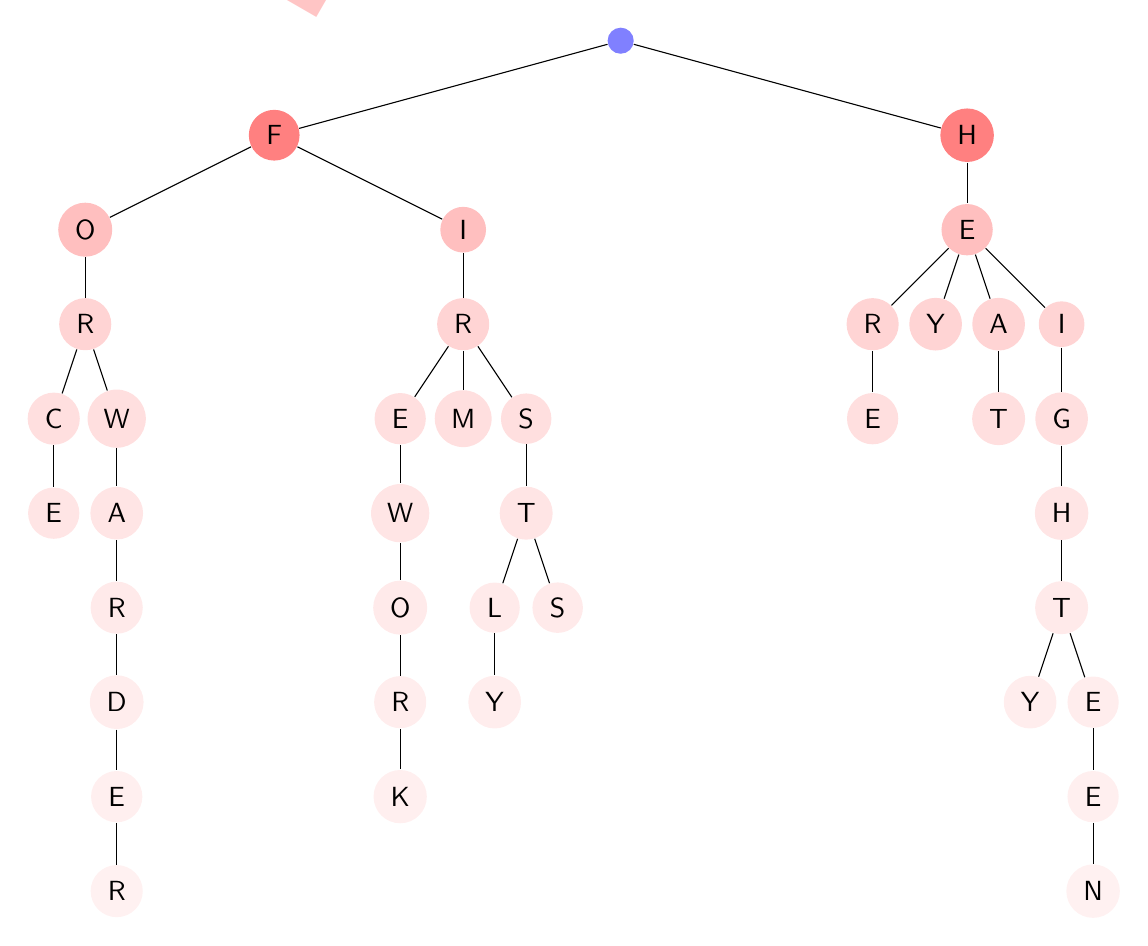
\begin{tikzpicture}[scale=0.8]
\node [circle, fill=blue!50]{}[sibling distance=11cm]
	child{node[circle, fill=red!50.000000]{F}[sibling distance=6cm]
		child{node[circle, fill=red!25.000000]{O}[sibling distance=1cm]
			child{node[circle, fill=red!16.666667]{R}[sibling distance=1cm]
				child{node[circle, fill=red!12.500000]{C}[sibling distance=1cm]
					child{node[circle, fill=red!10.000000]{E}[sibling distance=1cm]
					}
				}
				child{node[circle, fill=red!12.500000]{W}[sibling distance=1cm]
					child{node[circle, fill=red!10.000000]{A}[sibling distance=1cm]
						child{node[circle, fill=red!8.333333]{R}[sibling distance=1cm]
							child{node[circle, fill=red!7.142857]{D}[sibling distance=1cm]
								child{node[circle, fill=red!6.250000]{E}[sibling distance=1cm]
									child{node[circle, fill=red!5.555556]{R}[sibling distance=1cm]
									}
								}
							}
						}
					}
				}
			}
		}
		child{node[circle, fill=red!25.000000]{I}[sibling distance=1cm]
			child{node[circle, fill=red!16.666667]{R}[sibling distance=1cm]
				child{node[circle, fill=red!12.500000]{E}[sibling distance=1cm]
					child{node[circle, fill=red!10.000000]{W}[sibling distance=1cm]
						child{node[circle, fill=red!8.333333]{O}[sibling distance=1cm]
							child{node[circle, fill=red!7.142857]{R}[sibling distance=1cm]
								child{node[circle, fill=red!6.250000]{K}[sibling distance=1cm]
								}
							}
						}
					}
				}
				child{node[circle, fill=red!12.500000]{M}[sibling distance=1cm]
				}
				child{node[circle, fill=red!12.500000]{S}[sibling distance=1cm]
					child{node[circle, fill=red!10.000000]{T}[sibling distance=1cm]
						child{node[circle, fill=red!8.333333]{L}[sibling distance=1cm]
							child{node[circle, fill=red!7.142857]{Y}[sibling distance=1cm]
							}
						}
						child{node[circle, fill=red!8.333333]{S}[sibling distance=1cm]
						}
					}
				}
			}
		}
	}
	child{node[circle, fill=red!50.000000]{H}[sibling distance=1cm]
		child{node[circle, fill=red!25.000000]{E}[sibling distance=1cm]
			child{node[circle, fill=red!16.666667]{R}[sibling distance=1cm]
				child{node[circle, fill=red!12.500000]{E}[sibling distance=1cm]
				}
			}
			child{node[circle, fill=red!16.666667]{Y}[sibling distance=1cm]
			}
			child{node[circle, fill=red!16.666667]{A}[sibling distance=1cm]
				child{node[circle, fill=red!12.500000]{T}[sibling distance=1cm]
				}
			}
			child{node[circle, fill=red!16.666667]{I}[sibling distance=1cm]
				child{node[circle, fill=red!12.500000]{G}[sibling distance=1cm]
					child{node[circle, fill=red!10.000000]{H}[sibling distance=1cm]
						child{node[circle, fill=red!8.333333]{T}[sibling distance=1cm]
							child{node[circle, fill=red!7.142857]{Y}[sibling distance=1cm]
							}
							child{node[circle, fill=red!7.142857]{E}[sibling distance=1cm]
								child{node[circle, fill=red!6.250000]{E}[sibling distance=1cm]
									child{node[circle, fill=red!5.555556]{N}[sibling distance=1cm]
									}
								}
							}
						}
					}
				}
			}
		}
	}
;
\end{tikzpicture}

}

Le diagramme précédent a été créé par un programme développé en parallèle qui permet la création d'arbres visuels à partir d'un trie. Attention, cela n'est lisible que pour des arbres de petite taille (au delà, les branches se chevauchent). Cette illustration m'a permis de comprendre l'ensemble des proprités implémentées et de vérifier que tout état correct aisément.

On peut représenter comment le trie retrouve un mot visuellement. Cette fonction a été codée pour transformer le \type{trie} en \textit{tikz}. Ainsi, on peut retrouver le mot comme suit lettre par lettre en parcourant le trie.\\

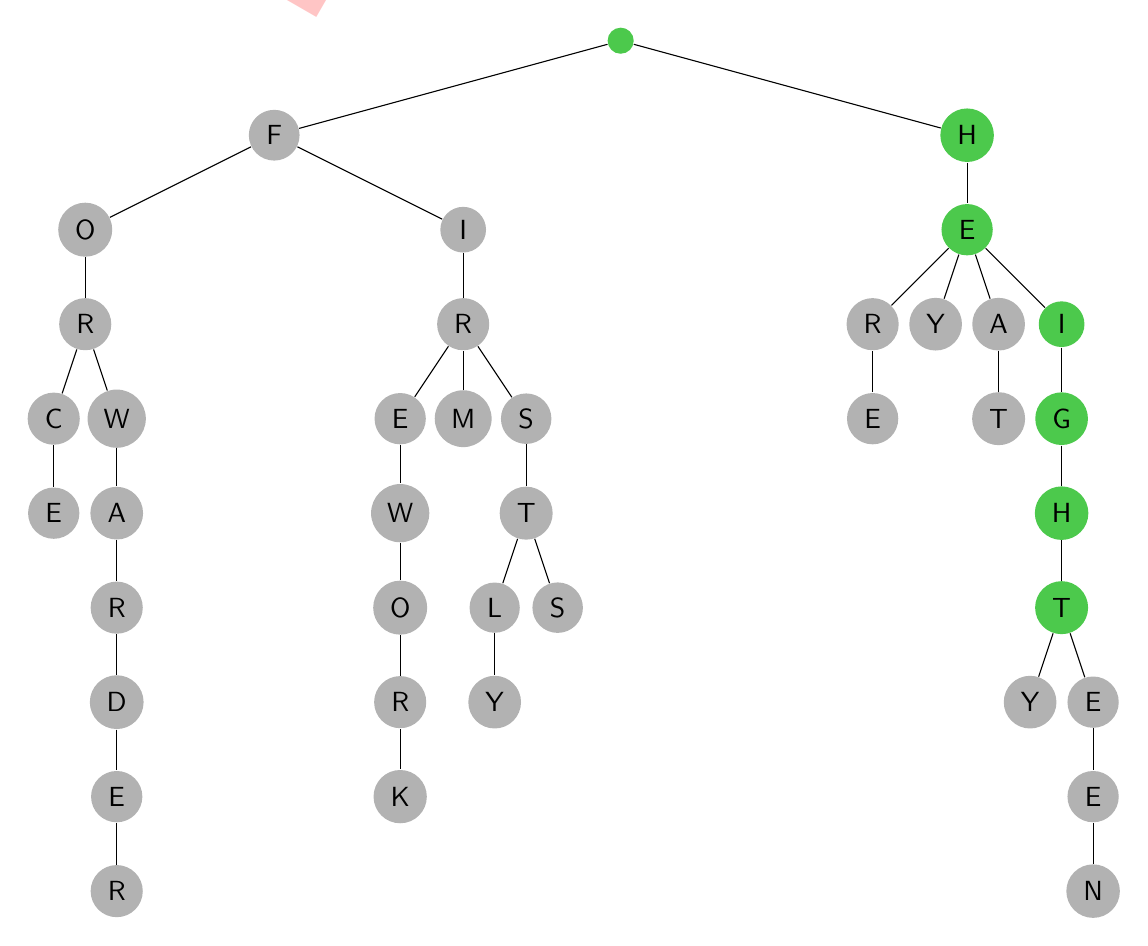
\begin{tikzpicture}[scale=0.8]
\node [circle, fill=green!70!black!70]{}[sibling distance=11cm]
	child{node[circle, fill=black!30]{F}[sibling distance=6cm]
		child{node[circle, fill=black!30]{O}[sibling distance=1cm]
			child{node[circle, fill=black!30]{R}[sibling distance=1cm]
				child{node[circle, fill=black!30]{C}[sibling distance=1cm]
					child{node[circle, fill=black!30]{E}[sibling distance=1cm]
					}
				}
				child{node[circle, fill=black!30]{W}[sibling distance=1cm]
					child{node[circle, fill=black!30]{A}[sibling distance=1cm]
						child{node[circle, fill=black!30]{R}[sibling distance=1cm]
							child{node[circle, fill=black!30]{D}[sibling distance=1cm]
								child{node[circle, fill=black!30]{E}[sibling distance=1cm]
									child{node[circle, fill=black!30]{R}[sibling distance=1cm]
									}
								}
							}
						}
					}
				}
			}
		}
		child{node[circle, fill=black!30]{I}[sibling distance=1cm]
			child{node[circle, fill=black!30]{R}[sibling distance=1cm]
				child{node[circle, fill=black!30]{E}[sibling distance=1cm]
					child{node[circle, fill=black!30]{W}[sibling distance=1cm]
						child{node[circle, fill=black!30]{O}[sibling distance=1cm]
							child{node[circle, fill=black!30]{R}[sibling distance=1cm]
								child{node[circle, fill=black!30]{K}[sibling distance=1cm]
								}
							}
						}
					}
				}
				child{node[circle, fill=black!30]{M}[sibling distance=1cm]
				}
				child{node[circle, fill=black!30]{S}[sibling distance=1cm]
					child{node[circle, fill=black!30]{T}[sibling distance=1cm]
						child{node[circle, fill=black!30]{L}[sibling distance=1cm]
							child{node[circle, fill=black!30]{Y}[sibling distance=1cm]
							}
						}
						child{node[circle, fill=black!30]{S}[sibling distance=1cm]
						}
					}
				}
			}
		}
	}
	child{node[circle, fill=green!70!black!70]{H}[sibling distance=1cm]
		child{node[circle, fill=green!70!black!70]{E}[sibling distance=1cm]
			child{node[circle, fill=black!30]{R}[sibling distance=1cm]
				child{node[circle, fill=black!30]{E}[sibling distance=1cm]
				}
			}
			child{node[circle, fill=black!30]{Y}[sibling distance=1cm]
			}
			child{node[circle, fill=black!30]{A}[sibling distance=1cm]
				child{node[circle, fill=black!30]{T}[sibling distance=1cm]
				}
			}
			child{node[circle, fill=green!70!black!70]{I}[sibling distance=1cm]
				child{node[circle, fill=green!70!black!70]{G}[sibling distance=1cm]
					child{node[circle, fill=green!70!black!70]{H}[sibling distance=1cm]
						child{node[circle, fill=green!70!black!70]{T}[sibling distance=1cm]
							child{node[circle, fill=black!30]{Y}[sibling distance=1cm]
							}
							child{node[circle, fill=black!30]{E}[sibling distance=1cm]
								child{node[circle, fill=black!30]{E}[sibling distance=1cm]
									child{node[circle, fill=black!30]{N}[sibling distance=1cm]
									}
								}
							}
						}
					}
				}
			}
		}
	}
;
\end{tikzpicture}



\subsection{Main counting function}
J'ai choisi de ne pas restreindre le dictionnaire outre mesure en forçant par exemple une suppression des accents, une casse spéciale pour les lettres... En effet, le \textit{trie} étant construit à partir d'un dictionnaire donné et que ce dernier est également utilisé pour l'extraction et la validation des mots, tous les mots partagent les mêmes caractères.

\begin{lstlisting}[language=Python, caption=Test all permutations]
def word_game_main_function(self, letters_list: list[str]) -> tuple[int, list[str]]:
    '''Return words built by given letters'''
    counter = 0
    words = []
    for i in range(3, len(letters_list) + 1):
        for permutation in permutations(letters_list, i):
            word = ''.join(permutation)
            if self.search(word):
                counter += 1
                words.append(word)
    return counter, words
\end{lstlisting}

La ligne du programme \verb|permutations(letters_list , i)| permet de générer toutes les permutations possibles grâce à la lib \verb|permutations| de \verb|itertools| de longueur $i$. Attention neanmoins à la complexité de cette opération.\\

Let say we have a word $W$ of $m$ letters.
The number of subwords of length k in an m-letter word can be calculated using the combination formula. For a word of m letters, there are C(m, k) subwords of length k, where C(m, k) represents the number of combinations of m elements taken k to k. The formula for C(m, k) is :
$$C(m, k) = \dfrac{m!}{k!(m - k)!}$$
Therefore, the total number of possible subwords in a word of m letters is the sum of the number of subwords of each length:
\begin{equation}
\text{Total number of subwords} = \sum_{k=3}^{m}C(m, k)
\label{eq:number_of_combination}
\end{equation}
Please note that this approach starts counting word from 3 letters and includes the word itself (of length m).
If you need a more specific answer, please provide the length m of the word you have and the more detailed context of what you mean by "subwords".
\begin{figure}[h]
    \centering
    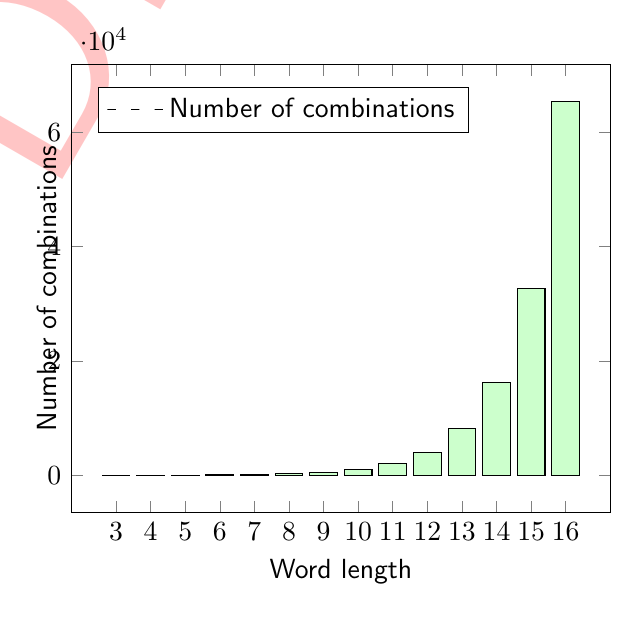
\begin{tikzpicture}
        \begin{axis}[
            xlabel=Word length,
            ylabel=Number of combinations,
            ylabel style={yshift=-10pt},
            xtick=data,
            legend style={at={(0.05,0.95)},anchor=north west}
            ]
        \addplot[ybar, bar width=10pt, fill=green!20]
            coordinates {
                (3, 0)
                (4, 4)
                (5, 15)
                (6, 41)
                (7, 98)
                (8, 218)
                (9, 465)
                (10, 967)
                (11, 1980)
                (12, 4016)
                (13, 8099)
                (14, 16277)
                (15, 32646)
                (16, 65398)
                };
        \legend{Number of combinations} 
        \end{axis}
    \end{tikzpicture}
\end{figure}

Comme chaque mot généré passera dans la machine, il peut être intéressant de diminuer au maximum la complexité unitaire de chacun des tests. On peut penser à stocker les mots qui ne sont pas dans l'arbre dans une liste (au moins leur radical) pour erradiquer tous les mots d'une même famille. Cependant, cette technique impose la création d'un nouveau trie et n'est donc pas satisfaisante.

\subsection{Interactive function}
\begin{itemize}
    \item Pour lancer le mode \textit{Interactive}, il faut régler la variable \verb|MODE_AUTO| à \verb|False|
    \item On peut ensuite régler l'input utilisateur dans l'appel de la fonction :
    \begin{lstlisting}[language=Python]
    results = manual_mode(trie, ['f', 'o', 'r', 'c', 'e'])
    \end{lstlisting}

    \item On peut ensuite lancer le programme en ligne de commande (sans oublier d'activer le \verb|venv|) :
    \begin{lstlisting}
    python3 word_challenge.py
    \end{lstlisting}
\end{itemize}

\subsection{Automatic execution}
\begin{itemize}
    \item Pour lancer le mode \textit{Automatic}, il faut régler la variable \verb|MODE_AUTO| à \verb|True|
    \item On peut ensuite régler le nombre de lettres à tenter dans la ligne suivantes :
    \begin{lstlisting}[language=Python]
    results = automated_mode(trie, 9)
    \end{lstlisting}

    \item On peut ensuite lancer le programme en ligne de commande (sans oublier d'activer le \verb|venv|) ET de renseigner un nombre de mots en ligne de commande :
    \begin{lstlisting}[language=Bash]
    python3 word_challenge.py 100
    \end{lstlisting}
\end{itemize}
Philosophie du programme :
\begin{itemize}
    \item L'utilisateur rentre en CLI un nombre de mots à tester
    \item Après avoir sélectionné un mot aléatoire dans le dictionnaire, le programme mélange aléatoirement les lettres (mises sous forme de liste) avec la fonction \verb|random.shuffle|
    \item Cette liste en donnée à la méthode \verb|word_game_main_function| qui retourne le compteur de subwords trouvés dans cette liste de lettres.
    \item Ces compteurs sont ensuite affichés dans un tableau en CLI et stockés dans un fichier \verb|.json|
\end{itemize}

\begin{table}[!ht]
    \centering
    \begin{tabular}{|c|c|c|c|}
        \hline
        Iteration & Initial length & CPU time & Word counter \\ \hline
        0 & 8 & 0.020746946334838867 & 72 \\ 
        1 & 10 & 1.9368188381195068 & 150 \\
        2 & 9 & 0.18332123756408691 & 120 \\ 
        3 & 5 & 0.00010991096496582031 & 11 \\ 
        ... & ~ & ~ & ~ \\ 
        49 & 11 & 22.33514976501465 & 721 \\ 
        \hline
        \hline
        AVG: & - & 0.989194917678833 & 71.22 \\ 
        \hline
    \end{tabular}
    \caption{Sample performances}
\end{table}

\subsubsection{Interact with dictionary}
\paragraph{Select random word}
Pour récupérer des mots aléatoires, il est nécessaire de choisir une ligne random et d'extraire le mot correspondant. Pour cela, on ouvre le fichier, on calcule le nombre de lignes total du dictionnaire (avec une simple fonction \verb|sum|), puis on extrait ensuite la seule ligne qui porte cet indice (par énumération). On récupère quelque chose de la forme \verb|future:121844371|. On extrait ensuite le mot avec la méthode suivante :
\begin{lstlisting}[language=Python]
word = line.strip().split(':')[0]
\end{lstlisting}
Une autre méthode a été utilisée avec une \textit{regex}: \verb|r'^(?:[a-zA-Z]+)'|

Pour sélectionner un mot d'une longueur définie, on s'appuie sur un \type{Trie}. On peut parcourir aléatoirement le \type{Trie} jusqu'à obtenir un mot d'une longueur voulue pour laquelle la dernière lettre possède l'attribut \verb|is_end_word|. On peut également sélectionner un mot aléatoirement jusqu'à obtenir un mot de la longueur désirée. Cela sera plus long, mais relativement négligeable comparé à l'effort nécessaire à implémenter l'autre méthode.\\


Les fonctions suivantes sont dans le fichier \verb|set_dictionary|.
\paragraph{Build trie with dictionary words}
De la même manière, et comme on en aura besoin dans la suite, on peut construire un trie avec l'ensemble des mots du dictionnaire pour l'utiliser par la suite dans la recherche de mots. On se repose alors sur les méthodes implémentées dans les structures de données \type{Trie} : comme la méthode \verb|insert_word| que l'on va itérer sur chacun des mots du dictionnaire. Cela donne quelque chose comme ça :
\begin{lstlisting}[language=Python]
def build_trie(file_path: str) -> Trie:
    '''Get random line from a goven file'''
    dictionary_trie = Trie()

    with open(file_path, 'r') as file:
        for line in file:
            dictionary_trie.insert_word(line.strip().split(':')[0])

    return dictionary_trie
\end{lstlisting}

\paragraph{Get alphabet}
Plus tard (dans l'exercice Wordle), nous aurons besoin de construire des mots à partir d'un alphabet. Pour utilsier les bonnes lettres dans cette étape, nous avons besoin d'avoir le même dictionnaire que celui utilisé pour vérifier la présence des mots dans le dictionnaire. Ainsi, en sélectionnant les lettres, nous nous assurons d'avoir les mêmes lettres. Avec cette façon, nous nous assurons de pouvoir comparer des mots peu importe le dictionnaire. Par exemple, nous pourrons à terme également utiliser des symboles non alphanumériques.\\

Nous utilisons une structure \type{set} car cela correspond exactement à ce que nous souhaitons en terme d'ajout des lettres. En effet, une lettre n'est ajoutée à l'alphabet seulement si elle n'est pas déjà dedans.\label{set}
L'alphabet fini $\Sigma$ est donc défini dynamiquement en extrayant l'ensemble des caractères de l'ensemble des mots du dictionnaire :
$$\Sigma = \{\sigma_i\}_{i\in[1, m]},\; m\geqslant 2$$
Soit $D$ le dictionnaire et $w$ un mot de ce dictionnaire, $c$ une lettre/caractère:
$$\Sigma = \bigcup_{w\in D}\{c\in w\}$$

\subsubsection{Performances}
Avant de tester les performances, nous devons analyser les données que nous avons pour être certain que le dictionnaire ne va pas brider notre analyse. On se propose alors d'afficher la quantité de chacun des mots par taille de mot :
\begin{figure}[h]
    \centering
    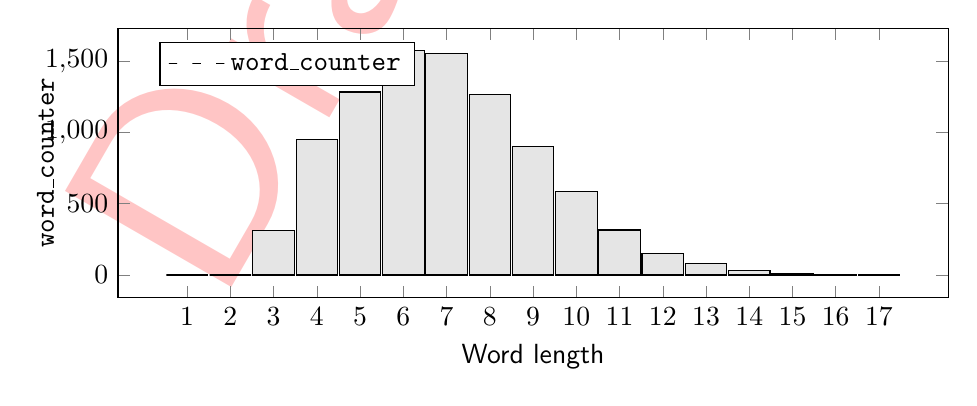
\begin{tikzpicture}
        \begin{axis}[
            xlabel=Word length,
            width=\linewidth,
            height=5cm,
            ylabel=\texttt{word\_counter},
            ylabel style={yshift=-10pt},
            xtick=data,
            legend style={at={(0.05,0.95)},anchor=north west}
            ]
        \addplot[ybar, bar width=15pt, fill=gray!20]
            coordinates {
                (1, 0)
                (2, 0)
                (3, 312)
                (4, 950)
                (5, 1285)
                (6, 1575)
                (7, 1557)
                (8, 1267)
                (9, 904)
                (10, 584)
                (11, 316)
                (12, 153)
                (13, 79)
                (14, 31)
                (15, 11)
                (16, 4)
                (17, 2)
                };
        \legend{ \texttt{word\_counter} } 
        \end{axis}
    \end{tikzpicture}
\end{figure}

Pour tester les performances de cet algorithme, nous utiliserons le mode automatique exclusivement. J'ai choisi de séparer l'exécution et le traitement des données en deux parties : récupérer les performances et analyser ensuite. Il faut donc extraire les performances avec la commande \verb|python3 word_challenge.py 100| en faisant attention à régler la longueur du mot à $0$ pour éviter de brider le programme avec une certaine longueur.
On peut ensuite exécuter le programme annexe de génération des histogrammes :
\begin{lstlisting}
python3 additional_algorithms/print_word_challenge_perf.py
\end{lstlisting}
Cela crée un fichier \verb|.tex| dans le dossier images du dossier documentation avec le graphe en question.

\begin{figure}[h]
    \centering

    \begin{subfigure}[b]{0.45\textwidth}
        \centering
        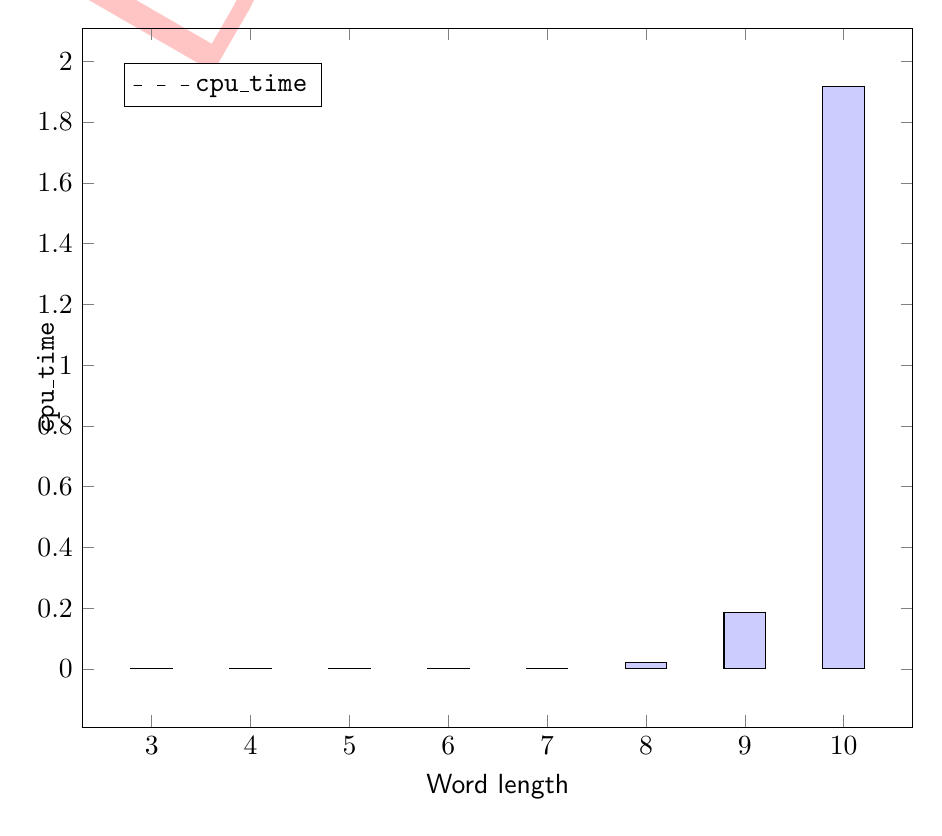
\begin{tikzpicture}
            \begin{axis}[
                xlabel=Word length,
                ylabel=\texttt{cpu\_time},
                ylabel style={yshift=-15pt},
                xtick=data,
                width=\linewidth,
                legend style={at={(0.05,0.95)},anchor=north west},
                ]
            \addplot[ybar, bar width=15pt, fill=blue!20]
                coordinates {
                    (3, 5.6425730387369794e-06)(4, 1.9073486328125e-05)(5, 8.714900297277113e-05)(6, 0.0004047552744547526)(7, 0.0025780797004699707)(8, 0.02060066952424891)(9, 0.18696789308027786)(10, 1.9171473185221355)
                    };
            \legend{ \texttt{cpu\_time} } 
            \end{axis}
        \end{tikzpicture}
    \end{subfigure}
    % \hfill
    \begin{subfigure}[b]{0.45\textwidth}
        \centering
        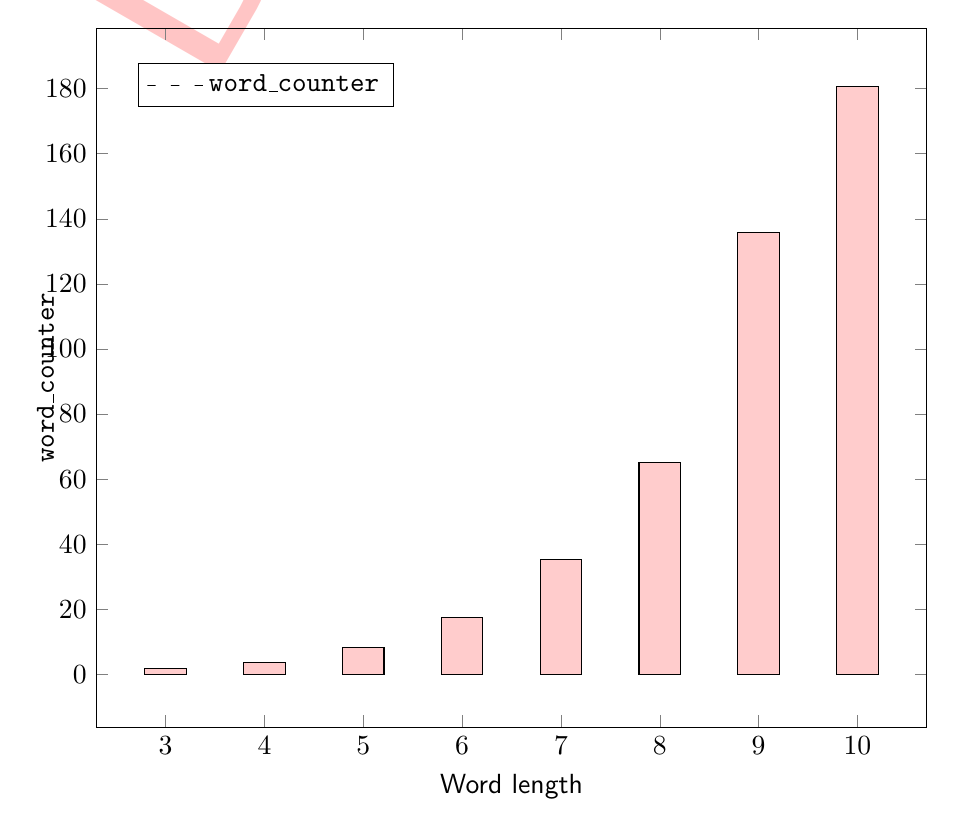
\begin{tikzpicture}
            \begin{axis}[
                xlabel=Word length,
                width=\linewidth,
                ylabel=\texttt{word\_counter},
                ylabel style={yshift=-10pt},
                xtick=data,
                legend style={at={(0.05,0.95)},anchor=north west}
                ]
            \addplot[ybar, bar width=15pt, fill=red!20]
                coordinates {
                    (3, 1.6666666666666667)(4, 3.7)(5, 8.294117647058824)(6, 17.428571428571427)(7, 35.25)(8, 65.23529411764706)(9, 135.9090909090909)(10, 180.66666666666666)
                    };
            \legend{ \texttt{word\_counter} } 
            \end{axis}
        \end{tikzpicture}
    \end{subfigure}
    \caption{Performances testing through process}
\end{figure}
Cette différence d'évolution s'explique par la construction même des mots. Il y a certes plus de lettres disponibles, mais cela crée beaucoup plus de mots qui n'existent pas dans le dictionnaire. On pourrait s'amuser à calculer la proportion de mots valides et non valides parmi toutes les permutations proposées par un set de lettres.

On remarque alors qu'avec 12 lettres ou plus, le programme est très très lent et ne permet pas de converger rapidement. En effet, l'équation \ref{eq:number_of_combination} donne pour 12 caractères 
\subsubsection{Improvements done}

\section{Wordle}
\begin{exercise_description}{Wordle}
    In Wordle (\url{https://en.wikipedia.org/wiki/Wordle}) the user can choose to play as \textit{keeper} or as \textit{guesser}. The length $\ell$ of the secret word is defined at the beginning of the game. When playing as \textit{guesser}, the program chooses a secret word of length $\ell$ and for each round the player writes a valid word of length $\ell$ and the computer outputs a string of digits with the following meaning: 0=the corresponding letter does not occur in the secret word, 1=the corresponding letter occurs in the secret word but not at that position, and 2=the corresponding letter occurs at that position. For example, if the secret word were \verb|WORDS| and the current guess were \verb|WHERE|, the program should output \verb|20010|, the \verb|W| was correctly guessed and the \verb|R| is on the secret word, but it is not in the fourth position. The game ends when the secret word is correctly guessed or some \verb|MAX_GUESSES| bound attained. When the player takes the role of the keeper, the computer will make the guesses and the user will give the answers (the strings of 0s, 1s, and 2's).\\

    Finally the program should offer an automatic mode in which the computer plays both as keeper and guesser (without cheating, the guesser function does not have access to the secret word, only its length $\ell$ and the history so far of guesses and answers). For the automatic mode, the human user fixes a length $\ell$ and a (large) number of games to be played. For each game, the keeper chooses a random word of length $\ell$ and a game is played between the keeper and the guesser. At the end, the program outputs the average number of rounds needed by the guesser to guess each secret word and the average CPU time to do it.     
\end{exercise_description}

\subsection*{Execute the programms}
\label{section:notice_wordle}
Pour tous les programmes, n'oubliez pas d'activer le \verb|venv|, puis lancer la commande suivante en réglant les paramètres comme suit :
\begin{lstlisting}[language=Python]
python3 wordle_game.py
\end{lstlisting}
\begin{itemize}
    \item Pour exécuter le programme guesser interactif, lancer la commande suivante:
\begin{lstlisting}[language=Python]
AUTOMATIC_MODE = False
GUESSER = True
KEEPER = False
\end{lstlisting}
    \item Pour exécuter le programme keeper interactif, lancer la commande suivante:
\begin{lstlisting}[language=Python]
AUTOMATIC_MODE = False
GUESSER = False
KEEPER = True
\end{lstlisting}
    \item Pour exécuter le programme automatique pour 1 seul puzzle
\begin{lstlisting}[language=Python]
AUTOMATIC_MODE = True
AUTOMATIC_MODE_GENERATOR = False
\end{lstlisting}
    \item Pour exécuter le programme automatique pour 200 points pour les 3 premières longueurs de mot $\ell\in\{3, 4, 5\}$
\begin{lstlisting}[language=Python]
AUTOMATIC_MODE = True
AUTOMATIC_MODE_GENERATOR = True
\end{lstlisting}
\end{itemize}

\subsection{Guesser mode}
\paragraph{Principle}
Le principe du jeu est défini dans l'énoncé. Je me contenterai donc d'expliquer l'implémentation et les choix de fonctions. Voici donc le cheminement qui sera utilisé par le programme. Le programme complet se trouve dans le fichier \verb|wordle_guesser.py|.
\begin{enumerate}
    \item Le programme choisit un mot aléatoire dans le dictionnaire fourni
    \item Il demande ensuite à l'utilisateur (ou au programme keeper dans la suite) de proposer un guess
    \item Il compare lettre par lettre si la lettre à cet indice est identique à celle au même indice dans le secret
    \item Si c'est le cas, alors le statut est fixé à 2 et enregistré dans une liste temporaire
    \item Si ce n'est pas le cas, il regarde si la lettre proposée est présente dans le secret (et renvoie 1 ou 0 en fonction de sa présence)
    \item Le programme rend finalement à l'utilisateur la concaténation des scores
    \item Ce programme se poursuit tant que l'utilisateur n'a pas réussi ou que l'utilisateur a dépassé le nombre de tentatives possible. 
\end{enumerate}
Dénomination : attention, dans la suite, le nom des programmes correspond à ce que doit réaliser l'utilisateur.
\paragraph{Human interaction}
On sépare la réception de l'intéraction homme/machine dans une fonction séparée pour pouvoir utiliser la fonction \verb|input| de python, puis parser le résultat pour l'inclure dans le programme par la suite.
\paragraph{Scores in array or string ?}
\begin{itemize}
    \item Travailler avec des chaines de caractère numériques n'est pas quelque chose de très simple pour l'analyse. On doit ensuite la parser pour en extraire les scores sous forme d'entiers. Cela fait l'objet d'une fonction intermédiaire. C'est parce qu'il ets demandé de travailler avec des chaines de caractère numériques type \verb|112001| qu'on le fait. C'est uniquement plus simple dans le cas de l'interaction homme/machine.
    \item Quoiqu'il arrive, à l'intérieur des programmes, les scores seront utilisés via des listes, par la traduction suivante par exemple :
\begin{lstlisting}[language=Python]
result_array = [0 for _ in range(word_length)]
\end{lstlisting}
        Puis ensuite la traduction inverse (transformation de la liste en chaîne de caractère) :
\begin{lstlisting}[language=Python]
''.join(map(str, result_array))
\end{lstlisting}
\end{itemize}

\subsection{Keeper mode}
Cette partie a été la plus complexe à modéliser pour que le jeu soit le plus rapide possible. En effet, une approche naïve de cet exercice serait de sélectionner des lettres aléatoires pour composer un mot, de le soumettre au test pour obtenir l'évaluation (en 0, 1 et 2) puis de tester un autre et ainsi de suite. Au fur et à mesure des tests, j'ai développé des nouvelles fonctionalités permettant de ne pas faire d'itérations inutiles, chose que l'on verra dans cette partie.

\subsubsection{Data structures used}
Chaque tentative est considérée comme une tentative a part entière relière aux précédentes informations reçues par le guesser. Ainsi, on peut capitaliser - comme le ferait un joueur normal - sur les tentatives précédentes. Pour cela, j'ai choisi de développer une nouvelle structure de donnée regroupant les informations utiles à la construction de chaque tentative (regroupant les lettres à essayer en priorité, celles qui mèneront à l'inutile...).

\paragraph{\type{WordLetter}} Il faut voir ce jeu comme une suite de tentatives de positionnement de lettres stratégiques. On peut donc créer une stratégie de résolution pour diminuer le nombre de tentatives.
\begin{itemize}
    \item Par exemple, on peut stocker toutes les lettres qui ont déjà été testées infructueusement pour ne pas les essayer de nouveau car cela mènerait à des tentatives inutiles. Attention cependant : en supprimant cette possibilité, on supprime également une grande quantité de mots valides qui nous auraient permis de déceler de nouvelles lettres potentielles.
    \item Je propose aussi d'implémenter dans le champ \verb|blocked_letter| un boolean qui permet de savoit si la lettre a été trouvée ou pas ($=2$). Dans ce cas, il est inutile de générer de nouvelles lettres.
\end{itemize}

\begin{figure}[h]
    \centering
    \begin{tikzpicture}
        \node[draw, rounded corners=2mm, inner sep = 0.2cm, fill=orange!0] { 
        \begin{tikzpicture} 
            \node[inner sep = 1mm] (title) { \Large{\bfseries WordLetter }}; 
            % \draw (title.south west) -- (title.south east);
            \node[at=(title.south), anchor=north, inner sep=3mm, align=left, fill=green!30!black!10, yshift=-0.2cm] (attributes) {
                \begin{minipage}{60mm}
                    \textbf{Attributes}\\
                    \small{0}: \verb|index|\\
\small{1}: \verb|past_letters|\\
\small{2}: \verb|score|\\
\small{3}: \verb|blocked_letter|\\
\small{4}: \verb|current_letter|
                \end{minipage} 
                };
            % \draw (attributes.north west) -- (attributes.north east);
            \node[at=(attributes.south), anchor=north, inner sep=3mm, align=left, fill=blue!10, yshift=-0.2cm] (methods) {
                \begin{minipage}{60mm}
                    \textbf{Methods}\\
                    \small{0}: \verb|add_letter_guess|\\
\small{1}: \verb|add_past_letter|\\
\small{2}: \verb|block_letter|\\
\small{3}: \verb|is_past_letter|\\
\small{4}: \verb|update_score|
                \end{minipage} 
                };
            % \draw (methods.north west) -- (methods.north east);
        \end{tikzpicture}
        }; 
    \end{tikzpicture}
    \caption{Class description - WordLetter }
    \label{class:WordLetter}
\end{figure}
\begin{itemize}
    \item On dote également cet objet de méthodes permettant de réaliser les fonctions précédentes comme ajouter une nouvelle lettre à la liste des lettres déjà testées
\end{itemize}

Pour conclure, les lettres deviennent des objets avec des propriétés les rendant intelligentes et non seulement des lettres au hasard dans un mot. Une partie de la logique du jeu est ainsi déportée dans la logique des lettres.


\paragraph{\type{Guess}} La structure de données vise à modéliser le raisonnement qu'on pourrait avoir en jouant au jeu Wordle en tant qu'humain. Les mots sont composés de lettres ordonnées qui donnent lieu a des essais/erreurs.
\begin{itemize}
    \item On choisit de modéliser le guess par une suite de $m$ mettres ordonnées par leur \verb|index|. Chaque lettres est initialisée au début du jeu et est nourrie ensuite. On donne aussi un alphabet au guess pour savoir dans quelle suite finie de lettres piocher pour constituer les mots.
    \item Les lettres déjà testées et qui ont mené à un échec ($=0$) sont stockées dans une liste noire (type : \type{set}) pour qu'elles ne soient pas testées de nouveau, peu importe la lettre \verb|bad_letters|. Ensuite, les lettres qui ont été testées mais mal positionnées ($=1$) sont stockées dans un \type{set} \verb|incorrect_position_letters|.
\end{itemize}
\begin{figure}[h]
    \centering
    \begin{tikzpicture}
        \node[draw, rounded corners=2mm, inner sep = 0.2cm, fill=orange!0] { 
        \begin{tikzpicture} 
            \node[inner sep = 1mm] (title) { \Large{\bfseries Guess }}; 
            % \draw (title.south west) -- (title.south east);
            \node[at=(title.south), anchor=north, inner sep=3mm, align=left, fill=green!30!black!10, yshift=-0.2cm] (attributes) {
                \begin{minipage}{60mm}
                    \textbf{Attributes}\\
                    \small{0}: \verb|letters|\\
\small{1}: \verb|length|\\
\small{2}: \verb|alphabet|\\
\small{3}: \verb|incorrect_position_letters|\\
\small{4}: \verb|bad_letters|\\
\small{5}: \verb|remaining_letters|\\
\small{6}: \verb|dictionary_trie|
                \end{minipage} 
                };
            % \draw (attributes.north west) -- (attributes.north east);
            \node[at=(attributes.south), anchor=north, inner sep=3mm, align=left, fill=blue!10, yshift=-0.2cm] (methods) {
                \begin{minipage}{60mm}
                    \textbf{Methods}\\
                    \small{0}: \verb|actualize_letter|\\
\small{1}: \verb|actualize_letters_informations|\\
\small{2}: \verb|display_word|\\
\small{3}: \verb|extract_random_letter|\\
\small{4}: \verb|generate_new_letters|\\
\small{5}: \verb|is_valid_word|\\
\small{6}: \verb|new_guess|
                \end{minipage} 
                };
            % \draw (methods.north west) -- (methods.north east);
        \end{tikzpicture}
        }; 
    \end{tikzpicture}
    \caption{Class description - Guess }
    \label{class:Guess}
\end{figure}

\textbf{Methods}
\begin{itemize}
    \setcounter{enumi}{-1}
    \item \verb|actualize_letter|: tester une nouvelle lettre pour un index donné
    \item \verb|actualize_letters_informations|: actualise le score de chaque lettre avant de tenter de deviner.
    \item \verb|display_word|: Affiche le mot qui est décomposé en \type{WordLetter} en une simple \type{string}.
\end{itemize}

\paragraph{\type{set}}
Comme évoqué dans le paragraphe \ref{set}, nous utilisons un set pour les lettres intertites et les lettres à positionner dans le mot car nous utilisons la propriété \verb|set.add()| qui permet de n'ajouter les informations seulement si elles le sont pas déjà inscrites.

\paragraph{\type{Trie}}
Pour chercher les mots et vérifier leur existence dans le dictionnaire, nous nous appuyons sur ce qui a été programmé dans la première partie de ce devoir. En effet, on indexe tous les mots du dictionnaire dans un trie avec la fonction \verb|build_trie| du dossier \verb|additional_algorithms|. Une fois que tous les mots sont inscrits dans le trie, on peut utilser la méthode codée pour vérifier l'existence du mot dans le trie \verb|trie.search(word: str)|.
Ainsi, la recherche des mots sera optimale.


\subsection{Automatic mode}

\subsubsection{Different modes}
Deux modes de résolution automatique ont été développé, le deuxième s'appuyant sur le premier. En effet, il est tout d'abord important de programmer la version automatique qui résout un puzzle imposé par le mode guesser. Ensuite, on peut chercher à scale cette résolution, d'où le deuxième programme.

\paragraph{Classic automatic mode}
Ce programme vise à interfacer à la fois le \textit{guesser} et le \textit{keeper}. En effet, le guesser répond 
\begin{lstlisting}[language=Python]
def guesser_automatic_mode(word_length: int = SECRET_LENGTH,
                            dictionary_path: str = DICTIONARY_PATH,
                            max_attempts: int = MAX_GUESSES
                          ) -> None:

    # Initialisation section : trie, alphabet, secret
    secret = ''
    trie = build_trie(dictionary_path)
    alphabet = set_alphabet(dictionary_path)

    # Define secret (generated)
    while len(secret) != word_length:
        secret = extract_informations(get_random_line(dictionary_path))

    # Set puzzle
    result_array = [0 for _ in range(word_length)]
    attempts = 0
    guess = Guess(word_length, trie, alphabet)

    # Solve puzzle
    while not all(num == 2 for num in result_array) and attempts < max_attempts:
        guess.new_guess([int(score) for score in result_array])
        new_guess = guess.display_word()
        result_array = check_guess(new_guess, secret)

        attempts += 1

    return {
    'solved': all(num == 2 for num in result_array),
    'attempts': attempts,
    'max_attempts': max_attempts,
    'size': word_length
    }

\end{lstlisting}

\paragraph{Generate data to analyse}
Pour chaque longueur de mot souhaité (de 3 à 5 ici dans l'exemple), on génère 200 résolutions de puzzle par le keeper. On stocke ensuite ce résultat dans un fichier json que l'on va enfin analyser avec le programme \verb|additional_algorithms/wordle_performance|. Cela permet de générer les coordonnées des courbes en partie performance. 
Cette solution a le mérite de pouvoir extraire beaucoup de données et de les traiter comme bon nous semble par la suite. Cela est notamment utile pour tracer les deux indicateurs dont nous avons besoin : le temps CPU et le nombre de tentatives nécessaires à trouver le mot.


\subsubsection{Performances}
Attention à un point en particulier. Dans cet exercice, j'ai choisi d'axer la performance sur le nombre minimum d'essais. Il aurait également pu être possible de favoriser la mesure du temps CPU en réalisant davantage d'essais.
\paragraph{How many attempts to solve the puzzle?}
On peut voir sur le graphique ci-dessus que la tendance dans le nombre d'essais pour résoudre les puzzle diminue avec la longueur de mot croissante. Cela s'explique de la manière suivante :
\begin{itemize}
    \item Plus de lettres dans un mot = plus de tentatives de lettres à chaque essais
    \item Donc plus de lettres marquées comme interdites
    \item Ces lettres ne sont donc plus utilisées et laissent la place à de nouvelles lettres susceptibles de correspondre (lettres générées aléatoirement)
    \item De même, en testant plus de lettres, on a plus d'informations sur les lettres avec le score 1.
\end{itemize}
\begin{figure}[h]
    \centering
    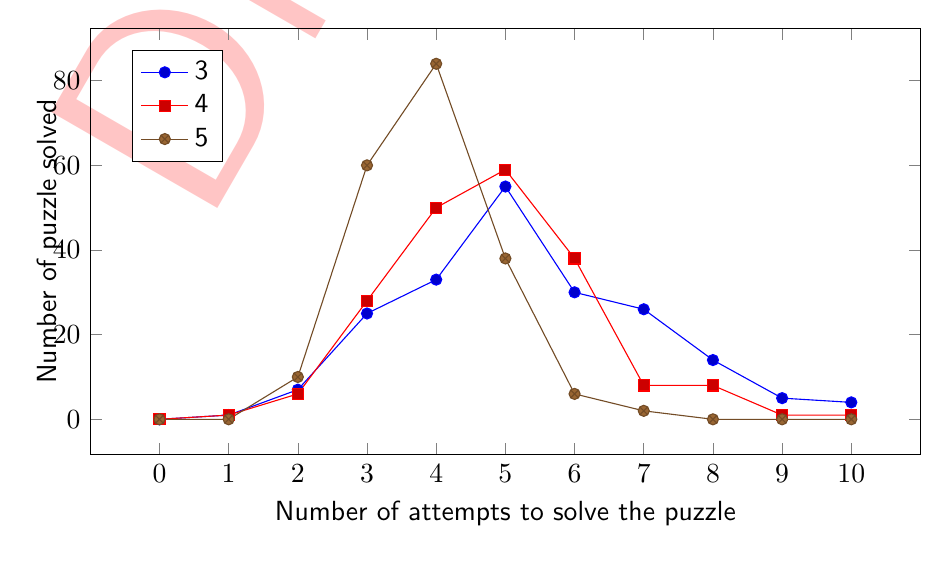
\begin{tikzpicture}
        \begin{axis}[
            xlabel=Number of attempts to solve the puzzle,
            width=\linewidth,
            height=7cm,
            ylabel=Number of puzzle solved,
            ylabel style={yshift=-10pt},
            xtick=data,
            legend style={at={(0.05,0.95)},anchor=north west}
            ]
        \addplot
            coordinates {
                (0, 0)
                (1, 1)
                (2, 7)
                (3, 25)
                (4, 33)
                (5, 55)
                (6, 30)
                (7, 26)
                (8, 14)
                (9, 5)
                (10, 4)
                };
        \addplot
            coordinates {
                (0, 0)
                (1, 1)
                (2, 6)
                (3, 28)
                (4, 50)
                (5, 59)
                (6, 38)
                (7, 8)
                (8, 8)
                (9, 1)
                (10, 1)
                };
            \addplot
            coordinates {
                (0, 0)
                (1, 0)
                (2, 10)
                (3, 60)
                (4, 84)
                (5, 38)
                (6, 6)
                (7, 2)
                (8, 0)
                (9, 0)
                (10, 0)
                };
                       
        \legend{3, 4, 5} 
        \end{axis}
    \end{tikzpicture}
    \caption{Automatic guesser performances measures}
\end{figure}
On remarque donc qu'en moyenne, le programme permet de générer la réponse à tous les challenges en moins de 5 coups. Cette performance est atteinte au prix du temps de calcul qui est relativement long pour les mots de grande taille.

\paragraph{How much CPU time needed to solve the puzzle?}
On peut aussi se demander, comme précisé précédemment combien de temps CPU, cette résolution représente. Cela se mesure simplement en chronométrant toute la partie résolution. La partie consacrée au guesser étant négligeable (car uniquement constante en temps), cela reflète quasi totalelent le temps CPU dédié au keeper. Ci après, on peut tracer, avec la commande suivante les graphiques de temps CPU pour les performances du keeper (attention à bien régler le programme sur l'utilisation en mode automatique, consignes ici : \ref{section:notice_wordle})
\begin{lstlisting}[language=Bash]
python3 wordle_game.py && python3 additional_algorithms/wordle_performance.py
\end{lstlisting}
Il est également possible de modifier la longueur des mots testés pour obtenir plus de performances, mais cela demanderait un calcul sur plusieurs heures.
\begin{figure}[h]
    \centering
    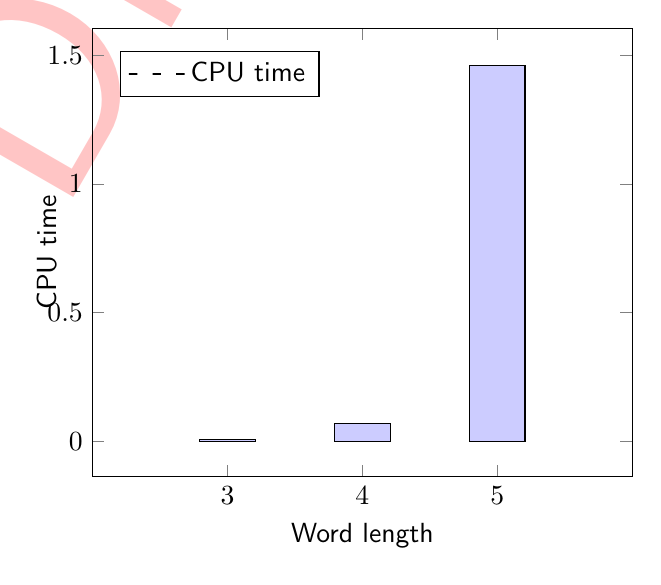
\begin{tikzpicture}
        \begin{axis}[
            xlabel=Word length,
            % width=\linewidth,
            % height=5cm,
            ylabel=CPU time,
            ylabel style={yshift=-10pt},
            xtick=data,
            xmin=2,
            xmax=6,
            legend style={at={(0.05,0.95)},anchor=north west}
            ]
        \addplot[ybar, bar width=20pt, fill=blue!20]
            coordinates {
                (3, 0.00882602334022522)
                (4, 0.06812063932418823)
                (5, 1.4601097178459168)
                };
        \legend{CPU time} 
        \end{axis}
    \end{tikzpicture}
\end{figure}


\section{Appendices}
\subsection{Personal feedback from this exercise}
cet exercice a été une réelle source d'apprentissage sur de nombreux points :
\begin{itemize}
    \item Programmation de projet complexe
    \item Rédaction de rapport technique
    \item Coder proprement en respectant les bonnes pratiques de développement
\end{itemize}
\subsection{Interfacing \textit{tikz} and programs}
\subsubsection{Produce dynamic tries with tikz}

\subsubsection{Draw class sumaries}
Plutot que de copier-coller et faire évoluer des morceaux de code séparément pour effectuer les mêmes tâches \textit{tikz}, j'ai choisi de construire une fonction python qui me permet de générer des résumés de chacune des classes utilisées dans les programmes. Cela permet donc de générer de nouveau toutes les illustrations du rapport si un fait évoluer un nom de variable ou qu'on les modifie. D'autre part, cela uniformise le rapport en pouvant changer les couleurs de tous les éléments d'un seul coup.



\newpage
\listoffigures
\lstlistoflistings
\listoftables
\end{document}






\begin{figure}[h]
    \centering
    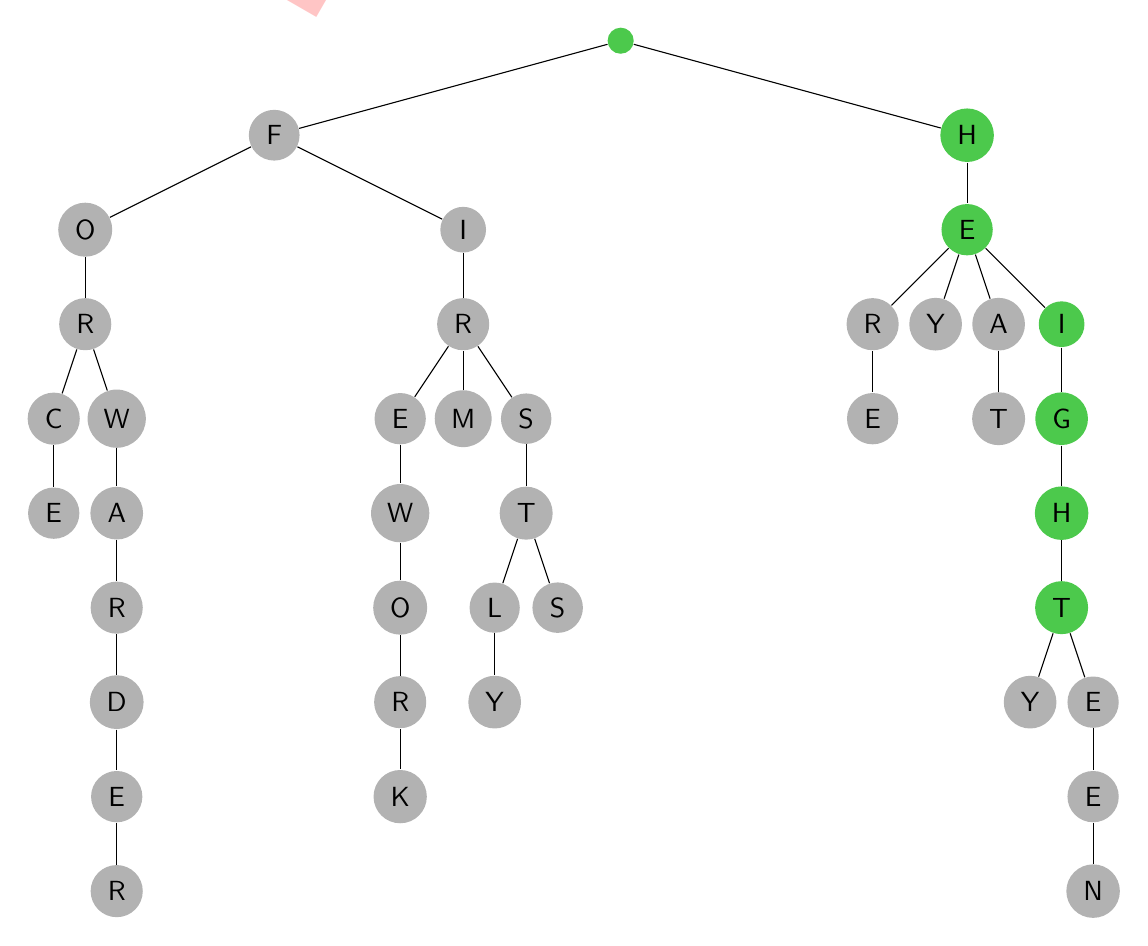
\begin{tikzpicture}[scale=0.8]
\node [circle, fill=green!70!black!70]{}[sibling distance=11cm]
	child{node[circle, fill=black!30]{F}[sibling distance=6cm]
		child{node[circle, fill=black!30]{O}[sibling distance=1cm]
			child{node[circle, fill=black!30]{R}[sibling distance=1cm]
				child{node[circle, fill=black!30]{C}[sibling distance=1cm]
					child{node[circle, fill=black!30]{E}[sibling distance=1cm]
					}
				}
				child{node[circle, fill=black!30]{W}[sibling distance=1cm]
					child{node[circle, fill=black!30]{A}[sibling distance=1cm]
						child{node[circle, fill=black!30]{R}[sibling distance=1cm]
							child{node[circle, fill=black!30]{D}[sibling distance=1cm]
								child{node[circle, fill=black!30]{E}[sibling distance=1cm]
									child{node[circle, fill=black!30]{R}[sibling distance=1cm]
									}
								}
							}
						}
					}
				}
			}
		}
		child{node[circle, fill=black!30]{I}[sibling distance=1cm]
			child{node[circle, fill=black!30]{R}[sibling distance=1cm]
				child{node[circle, fill=black!30]{E}[sibling distance=1cm]
					child{node[circle, fill=black!30]{W}[sibling distance=1cm]
						child{node[circle, fill=black!30]{O}[sibling distance=1cm]
							child{node[circle, fill=black!30]{R}[sibling distance=1cm]
								child{node[circle, fill=black!30]{K}[sibling distance=1cm]
								}
							}
						}
					}
				}
				child{node[circle, fill=black!30]{M}[sibling distance=1cm]
				}
				child{node[circle, fill=black!30]{S}[sibling distance=1cm]
					child{node[circle, fill=black!30]{T}[sibling distance=1cm]
						child{node[circle, fill=black!30]{L}[sibling distance=1cm]
							child{node[circle, fill=black!30]{Y}[sibling distance=1cm]
							}
						}
						child{node[circle, fill=black!30]{S}[sibling distance=1cm]
						}
					}
				}
			}
		}
	}
	child{node[circle, fill=green!70!black!70]{H}[sibling distance=1cm]
		child{node[circle, fill=green!70!black!70]{E}[sibling distance=1cm]
			child{node[circle, fill=black!30]{R}[sibling distance=1cm]
				child{node[circle, fill=black!30]{E}[sibling distance=1cm]
				}
			}
			child{node[circle, fill=black!30]{Y}[sibling distance=1cm]
			}
			child{node[circle, fill=black!30]{A}[sibling distance=1cm]
				child{node[circle, fill=black!30]{T}[sibling distance=1cm]
				}
			}
			child{node[circle, fill=green!70!black!70]{I}[sibling distance=1cm]
				child{node[circle, fill=green!70!black!70]{G}[sibling distance=1cm]
					child{node[circle, fill=green!70!black!70]{H}[sibling distance=1cm]
						child{node[circle, fill=green!70!black!70]{T}[sibling distance=1cm]
							child{node[circle, fill=black!30]{Y}[sibling distance=1cm]
							}
							child{node[circle, fill=black!30]{E}[sibling distance=1cm]
								child{node[circle, fill=black!30]{E}[sibling distance=1cm]
									child{node[circle, fill=black!30]{N}[sibling distance=1cm]
									}
								}
							}
						}
					}
				}
			}
		}
	}
;
\end{tikzpicture}


    \caption{Search path}
    \label{fig:search_path_pgm}
\end{figure}

\begin{figure}[h]
    \centering
    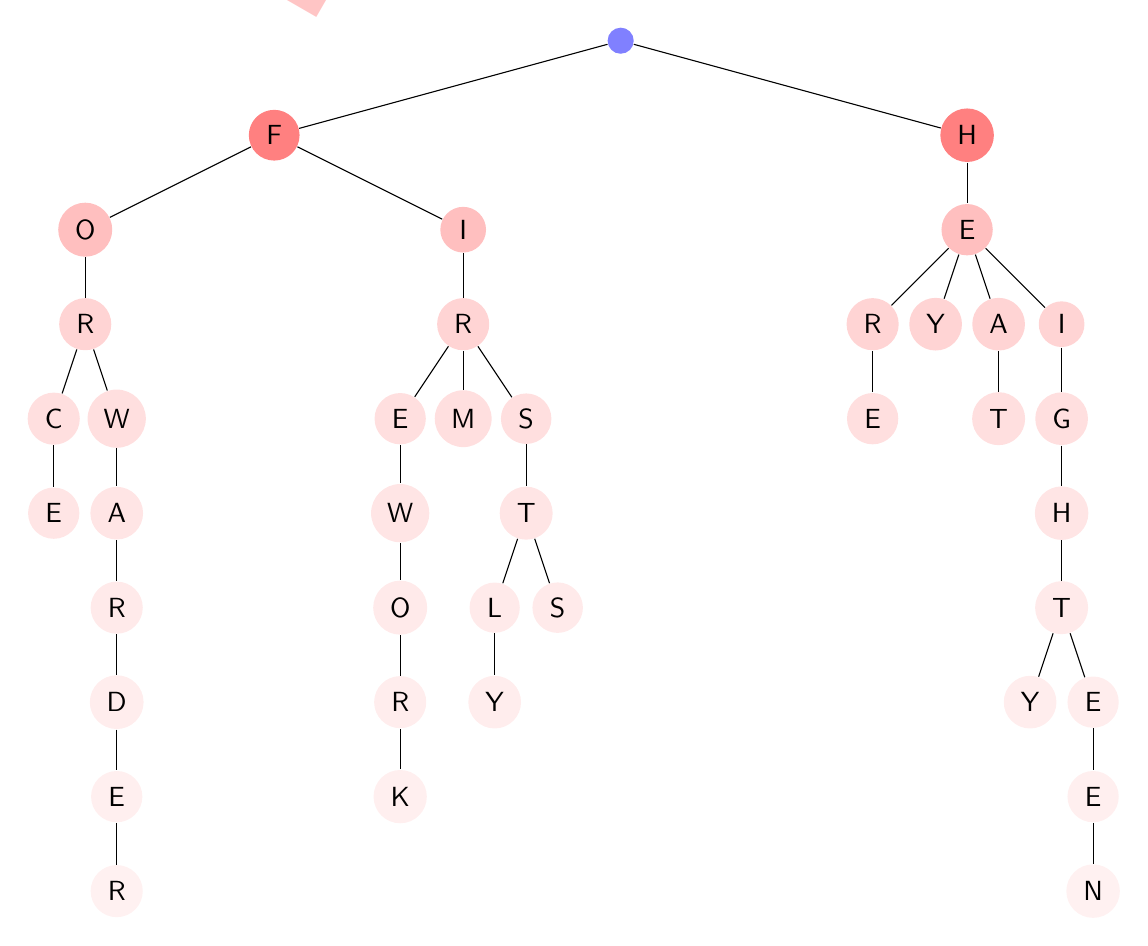
\begin{tikzpicture}[scale=0.8]
\node [circle, fill=blue!50]{}[sibling distance=11cm]
	child{node[circle, fill=red!50.000000]{F}[sibling distance=6cm]
		child{node[circle, fill=red!25.000000]{O}[sibling distance=1cm]
			child{node[circle, fill=red!16.666667]{R}[sibling distance=1cm]
				child{node[circle, fill=red!12.500000]{C}[sibling distance=1cm]
					child{node[circle, fill=red!10.000000]{E}[sibling distance=1cm]
					}
				}
				child{node[circle, fill=red!12.500000]{W}[sibling distance=1cm]
					child{node[circle, fill=red!10.000000]{A}[sibling distance=1cm]
						child{node[circle, fill=red!8.333333]{R}[sibling distance=1cm]
							child{node[circle, fill=red!7.142857]{D}[sibling distance=1cm]
								child{node[circle, fill=red!6.250000]{E}[sibling distance=1cm]
									child{node[circle, fill=red!5.555556]{R}[sibling distance=1cm]
									}
								}
							}
						}
					}
				}
			}
		}
		child{node[circle, fill=red!25.000000]{I}[sibling distance=1cm]
			child{node[circle, fill=red!16.666667]{R}[sibling distance=1cm]
				child{node[circle, fill=red!12.500000]{E}[sibling distance=1cm]
					child{node[circle, fill=red!10.000000]{W}[sibling distance=1cm]
						child{node[circle, fill=red!8.333333]{O}[sibling distance=1cm]
							child{node[circle, fill=red!7.142857]{R}[sibling distance=1cm]
								child{node[circle, fill=red!6.250000]{K}[sibling distance=1cm]
								}
							}
						}
					}
				}
				child{node[circle, fill=red!12.500000]{M}[sibling distance=1cm]
				}
				child{node[circle, fill=red!12.500000]{S}[sibling distance=1cm]
					child{node[circle, fill=red!10.000000]{T}[sibling distance=1cm]
						child{node[circle, fill=red!8.333333]{L}[sibling distance=1cm]
							child{node[circle, fill=red!7.142857]{Y}[sibling distance=1cm]
							}
						}
						child{node[circle, fill=red!8.333333]{S}[sibling distance=1cm]
						}
					}
				}
			}
		}
	}
	child{node[circle, fill=red!50.000000]{H}[sibling distance=1cm]
		child{node[circle, fill=red!25.000000]{E}[sibling distance=1cm]
			child{node[circle, fill=red!16.666667]{R}[sibling distance=1cm]
				child{node[circle, fill=red!12.500000]{E}[sibling distance=1cm]
				}
			}
			child{node[circle, fill=red!16.666667]{Y}[sibling distance=1cm]
			}
			child{node[circle, fill=red!16.666667]{A}[sibling distance=1cm]
				child{node[circle, fill=red!12.500000]{T}[sibling distance=1cm]
				}
			}
			child{node[circle, fill=red!16.666667]{I}[sibling distance=1cm]
				child{node[circle, fill=red!12.500000]{G}[sibling distance=1cm]
					child{node[circle, fill=red!10.000000]{H}[sibling distance=1cm]
						child{node[circle, fill=red!8.333333]{T}[sibling distance=1cm]
							child{node[circle, fill=red!7.142857]{Y}[sibling distance=1cm]
							}
							child{node[circle, fill=red!7.142857]{E}[sibling distance=1cm]
								child{node[circle, fill=red!6.250000]{E}[sibling distance=1cm]
									child{node[circle, fill=red!5.555556]{N}[sibling distance=1cm]
									}
								}
							}
						}
					}
				}
			}
		}
	}
;
\end{tikzpicture}


    \caption{Draw trie}
    \label{fig:draw_pgm}
\end{figure}



\section{Data structure}
\subsection{Tries implementation}


\section{Performances}
\begin{summary}
    Essai
\end{summary}


\section{Complexity and time preduction}


\begin{figure}
    \centering
    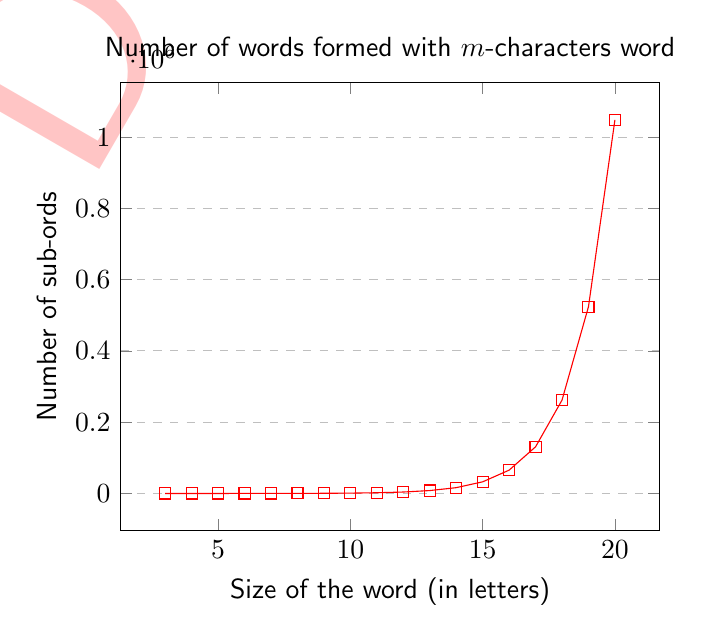
\begin{tikzpicture}
\begin{axis}[
    title={Number of words formed with $m$-characters word},
    xlabel={Size of the word (in letters)},
    ylabel={Number of sub-ords},
    % xmin=0, xmax=100,
    % ymin=0, ymax=120,
    % xtick={0,20,40,60,80,100},
    % ytick={0,20,40,60,80,100,120},
    legend pos=north west,
    ymajorgrids=true,
    grid style=dashed,
]

\addplot[
    color=red,
    mark=square,
    ]
    coordinates {
        (3, 0)
        (4, 4)
        (5, 15)
        (6, 41)
        (7, 98)
        (8, 218)
        (9, 465)
        (10, 967)
        (11, 1980)
        (12, 4016)
        (13, 8099)
        (14, 16277)
        (15, 32646)
        (16, 65398)
        (17, 130917)
        (18, 261971)
        (19, 524096)
        (20, 1048364)
    };
    
\end{axis}
\end{tikzpicture}

    \caption{A PGF histogram from \texttt{matplotlib}.}
\end{figure}

As a consequence, we have to find a way to decrease the number of 

\section{Ideas}
Change the programmation philosophy to:
\begin{itemize}
    \item Définition des fonctions de jeu par récurrence: appel de la fonction avec comme paramètres
        \begin{itemize}
            \item Mot à deviner (secret)
            \item Mot choisi par l'utilisateur
            \item Résultat (en terme de 0, 1, 2)
            \item Numéro de l'essais 
        \end{itemize}
        Cela permettra de faire appel aux fonctions par récurrence et de mutualiser les programmes de \textit{guesser} et de \textit{keeper}
    \item Passer en programmation par objet avec un objet pour :
        \begin{itemize}
            \item guesser
            \item keeper
            \item guess
            \item secret
            \item tentative
        \end{itemize}
\end{itemize}

\section{Best practices}
\begin{itemize}
    \item Description des fonctions avec docstring
    \item Ajout des typages pour les fonctions (aide à l'IDE)
    \item Mise en commun des fonctions identiques (factorisation)
    \item Tentative d'optimisation
\end{itemize}



\section{Objects}
\begin{figure}[h]
    \centering
    \begin{tikzpicture}
        \node[draw, rounded corners=2mm, inner sep = 0.2cm, fill=orange!0] { 
        \begin{tikzpicture} 
            \node[inner sep = 1mm] (title) { \Large{\bfseries Guess }}; 
            % \draw (title.south west) -- (title.south east);
            \node[at=(title.south), anchor=north, inner sep=3mm, align=left, fill=green!30!black!10, yshift=-0.2cm] (attributes) {
                \begin{minipage}{60mm}
                    \textbf{Attributes}\\
                    \small{0}: \verb|letters|\\
\small{1}: \verb|length|\\
\small{2}: \verb|alphabet|\\
\small{3}: \verb|incorrect_position_letters|\\
\small{4}: \verb|bad_letters|\\
\small{5}: \verb|remaining_letters|\\
\small{6}: \verb|dictionary_trie|
                \end{minipage} 
                };
            % \draw (attributes.north west) -- (attributes.north east);
            \node[at=(attributes.south), anchor=north, inner sep=3mm, align=left, fill=blue!10, yshift=-0.2cm] (methods) {
                \begin{minipage}{60mm}
                    \textbf{Methods}\\
                    \small{0}: \verb|actualize_letter|\\
\small{1}: \verb|actualize_letters_informations|\\
\small{2}: \verb|display_word|\\
\small{3}: \verb|extract_random_letter|\\
\small{4}: \verb|generate_new_letters|\\
\small{5}: \verb|is_valid_word|\\
\small{6}: \verb|new_guess|
                \end{minipage} 
                };
            % \draw (methods.north west) -- (methods.north east);
        \end{tikzpicture}
        }; 
    \end{tikzpicture}
    \caption{Class description - Guess }
    \label{class:Guess}
\end{figure}
\begin{figure}[h]
    \centering
    \begin{tikzpicture}
        \node[draw, rounded corners=2mm, inner sep = 0.2cm, fill=orange!0] { 
        \begin{tikzpicture} 
            \node[inner sep = 1mm] (title) { \Large{\bfseries Trie }}; 
            % \draw (title.south west) -- (title.south east);
            \node[at=(title.south), anchor=north, inner sep=3mm, align=left, fill=green!30!black!10, yshift=-0.2cm] (attributes) {
                \begin{minipage}{60mm}
                    \textbf{Attributes}\\
                    \small{0}: \verb|root|
                \end{minipage} 
                };
            % \draw (attributes.north west) -- (attributes.north east);
            \node[at=(attributes.south), anchor=north, inner sep=3mm, align=left, fill=blue!10, yshift=-0.2cm] (methods) {
                \begin{minipage}{60mm}
                    \textbf{Methods}\\
                    \small{0}: \verb|insert_word|\\
\small{1}: \verb|search|\\
\small{2}: \verb|word_game_main_function|
                \end{minipage} 
                };
            % \draw (methods.north west) -- (methods.north east);
        \end{tikzpicture}
        }; 
    \end{tikzpicture}
    \caption{Class description - Trie }
    \label{class:Trie}
\end{figure}
\begin{figure}[h]
    \centering
    \begin{tikzpicture}
        \node[draw, rounded corners=2mm, inner sep = 0.2cm, fill=orange!0] { 
        \begin{tikzpicture} 
            \node[inner sep = 1mm] (title) { \Large{\bfseries TrieNode }}; 
            % \draw (title.south west) -- (title.south east);
            \node[at=(title.south), anchor=north, inner sep=3mm, align=left, fill=green!30!black!10, yshift=-0.2cm] (attributes) {
                \begin{minipage}{60mm}
                    \textbf{Attributes}\\
                    \small{0}: \verb|children|\\
\small{1}: \verb|is_end_word|\\
\small{2}: \verb|value|\\
\small{3}: \verb|depth|
                \end{minipage} 
                };
            % \draw (attributes.north west) -- (attributes.north east);
            \node[at=(attributes.south), anchor=north, inner sep=3mm, align=left, fill=blue!10, yshift=-0.2cm] (methods) {
                \begin{minipage}{60mm}
                    \textbf{Methods}\\
                    \small{0}: \verb|leaves_counter_recursive|
                \end{minipage} 
                };
            % \draw (methods.north west) -- (methods.north east);
        \end{tikzpicture}
        }; 
    \end{tikzpicture}
    \caption{Class description - TrieNode }
    \label{class:TrieNode}
\end{figure}
\begin{figure}[h]
    \centering
    \begin{tikzpicture}
        \node[draw, rounded corners=2mm, inner sep = 0.2cm, fill=orange!0] { 
        \begin{tikzpicture} 
            \node[inner sep = 1mm] (title) { \Large{\bfseries WordLetter }}; 
            % \draw (title.south west) -- (title.south east);
            \node[at=(title.south), anchor=north, inner sep=3mm, align=left, fill=green!30!black!10, yshift=-0.2cm] (attributes) {
                \begin{minipage}{60mm}
                    \textbf{Attributes}\\
                    \small{0}: \verb|index|\\
\small{1}: \verb|past_letters|\\
\small{2}: \verb|score|\\
\small{3}: \verb|blocked_letter|\\
\small{4}: \verb|current_letter|
                \end{minipage} 
                };
            % \draw (attributes.north west) -- (attributes.north east);
            \node[at=(attributes.south), anchor=north, inner sep=3mm, align=left, fill=blue!10, yshift=-0.2cm] (methods) {
                \begin{minipage}{60mm}
                    \textbf{Methods}\\
                    \small{0}: \verb|add_letter_guess|\\
\small{1}: \verb|add_past_letter|\\
\small{2}: \verb|block_letter|\\
\small{3}: \verb|is_past_letter|\\
\small{4}: \verb|update_score|
                \end{minipage} 
                };
            % \draw (methods.north west) -- (methods.north east);
        \end{tikzpicture}
        }; 
    \end{tikzpicture}
    \caption{Class description - WordLetter }
    \label{class:WordLetter}
\end{figure}

\end{document}
